\section{Generiranje značajki}

Generiranje značajki je drugi podsustav spomenut u uvodnom dijelu, također
prikazan na slici \ref{pic:struktura_sustava}. Nakon što je omogućena akvizicija
zvučnih uzoraka, potrebno ih je obraditi kako bi se mogli predati neuronskoj mreži 
na klasifikaciju. Naime, modeli strojnog učenja (kao što je neuronska mreža) rade
s različitim primjerima podataka. Razlikovanje primjera temelji se na odredivanju
različitih značajki ulaznih podataka. Klasičan primjer koji se koristi kako bi se 
približio pojam značajki jest model predikcije cijene nekakve
nekretnine. U tom slučaju značajke koje bi model mogao koristiti su lokacija,
godina izgradnje, površina, razina energetske učinkovitosti i slično. Medutim, što
bi bile značajke našeg ulaznog toka signala? Možemo, ispostavit će se naivno, uzeti
amplitudu svake vrijednosti. U slučaju da promatramo period od jedne sekunde
signala s već spomenutim otipkavanjem od 16 kHz, broj značajki koje bi naš model
morao ”progutati” jest 16000. Obraditi toliku količinu podataka u jako kratkom
vremenu (sustav mora raditi bez konstantno i bez mrtvog vremena) na resursno
ograničenom sustavu kao što je mikrokontroler ne zvuči obećavajuće. Nekako sve 
upućuje na to da je potrebno na neki način prilagoditi ulazni signal, tj. izvući
iz signala bitne informacije i tako smanjiti veličinu podataka. 

\subsection{Model govora}
\label{sec:speech}

Kako bismo identificirali kojim značajkama bi bilo korisno opisati ljudski govor,
potrebno je na neki način modelirati nastanak glasa. Prilikom govorne komunikacije,
pluća govornika se pod djelovanjem mišića prsnog koša stišću i potiskuju zrak kroz
vokalni trakt čiji su glavni dijelovi prikazani na slici \ref{pic:glas}.

\begin{figure}[htb]
    \centering
    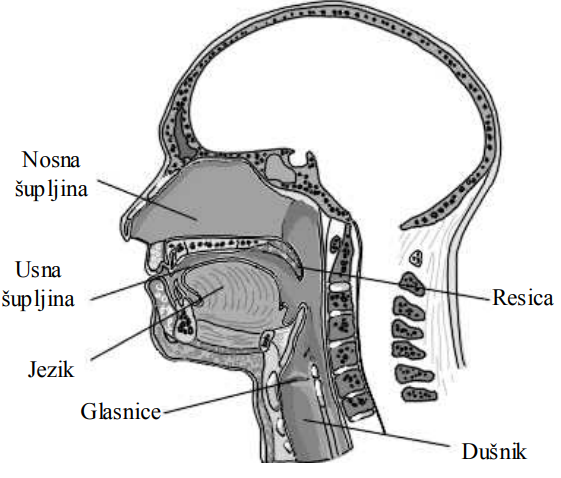
\includegraphics[width=0.6\linewidth]{Chapters/struktura_sustava/generiranje_znacajki/glas.png} 
    \caption{Presjek glave i osnovni dijelovi vokalnog trakta koji sudjeluju u produkciji govornog signala \cite{petrinovic2002}}
    \label{pic:glas}
\end{figure}

Glasnice (engl. glottis) su vrlo značajan organ u procesu formiranja govora. 
Ponašaju se kao mehanički
oscilator koji prelazi u stanje relaksacijskih oscilacija uslijed struje zraka iz pluća koja kroz njih
prolazi. Na frekvenciju njihovog titranja utječu brojni parametri, a među najznačajnijim su
pritisak zraka iz pluća na ulazu u glasnice i napetost samih glasnica.
Takvim periodičkim titranjem, glasnice formiraju periodičku struju zraka, tj. 
kvazi-periodične impulse (engl. glottal pulse) koja zatim prolaze kroz ostatak 
vokalnog trakta što vodi do stvaranja artikuliranih glasova. U slučaju da 
su glasnice potpuno opuštene, neće
doći do oscilacija i struja zraka iz pluća će neometano prolaziti kroz vokalni trakt 
(tada se ne formira kvazi-periodični impuls, nego je rezultat prolaska zraka kroz glasnice
slučajni šum, a rezultat cijelog procesa je stvaranje neartikuliranih glasova). 

S druge strane, vokalni trakt se ponaša kao filtar koji spektralno mijenja karakteristiku
pobudnog signala (engl. vocal tract frequency response). 
Geometrijom vokalnog trakta, koja se mijenja ovisno o položaju 
artikulatora kao što su jezik, usne, čeljust i resica, bit će određen ton (visina i
spektralni sastav) formiranog signala (govora) \cite{petrinovic2002}. 

Jednostavni model koji se koristi u području obrade prirodnog govora je da se on 
može prikazati kao izlaz iz linearnog, vremenski promjenjivog sustava čija se 
svojstva sporo mijenjaju s vremenom. Međutim, ako se promatraju dovoljno kratki
segmenti govornog signala, svaki se segment može učinkovito modelirati kao izlaz
iz linearnog, vremenski invarijantnog sustava pobuđenog bilo
kvazi-periodičnim impulsima bilo slučajnim šumom (engl. random noise signal).
Opisani sustav može se prikazati jednadžbom \ref{eq:govor}

\begin{equation}
    \label{eq:govor}
    X(f) = E(f) \cdot H(f)
\end{equation}

gdje je:
\begin{itemize}
    \item \(X(f)\) odziv sustava (govor),
    \item \(E(f)\) pobuda (kvazi-periodični impuls),
    \item \(H(f)\) prijenosna funkcija vokalnog trakta.
\end{itemize}

U vremenskoj domeni isti sustav može se prikazati jednadžbom \ref{eq:govor_vremenska}.
Množenju u frekvencijskoj domeni istovjetna je konvolucija u vremenskoj (i obratno!).

\begin{equation}
    \label{eq:govor_vremenska}
    x(t) = e(t) \ast h(t)
\end{equation}

Cilj ovakvog modeliranja je pronaći bitne informacije u govornom signalu. Pretpostavka na
kojoj se temelji daljnji rad je da je skoro sva informacija iz govornog signala sadržana
u prijenosnoj funkciji govornog trakta, tj. pobuda (kvazi-periodični impulsi) ostaje
konstantnna tijekom govora (veliko pojednostavljenje, međutim svi modeli na kojima
se temelji ovo područje zasnivaju na ovoj činjenici \cite{multiplier, emotion, sidhu2024mfcc}).
Zbog toga želimo pronaći način za 
razdvajanje tih dvaju elemenata modela. Ako primijenimo logaritamsku funkciju na
sustav opisan u frekvencijskoj domeni proizlazi \ref{eq:logaritam}.

\begin{equation}
    \label{eq:logaritam}
    \begin{aligned}
        \log(X(f)) &= \log(E(f) \cdot H(f)) \\
        \log(X(f)) &= \log(E(f)) + \log(H(f))
    \end{aligned}
\end{equation}

Prikazanim su uspješno razdvojeni elementi modela, tj. vidljiv je rastav na zbrojnike
ako se primijeni logaritamska skala. Na slici \ref{pic:rastav} prikazan je utjecaj
komponenata modela na konačni rezultat, a to je glas (engl. speech). 

\begin{figure}[htb]
    \centering
    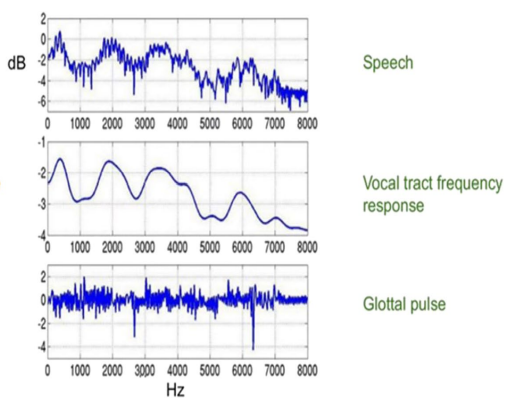
\includegraphics[width=0.6\linewidth]{Chapters/struktura_sustava/generiranje_znacajki/log.png} 
    \caption{Glasovni signal rastavljen na pobudu i odziv vokalnog trakta \cite{sidhu2024mfcc}}
    \label{pic:rastav}
\end{figure}

Jedino što preostaje je pronaći način za što efikasniji opis odziva vokalnog trakta. On će
u konačnici predstavljati zvučne zapise na kojima će model neuronske mreže biti treniran.
U području automatskog prepoznavanja govora te identifikaciji govornika uvelike se koriste
Mel kepstralni koeficijenti.


\subsection{MFCC}
\label{MFCCconstruction}
Mel kepstralni koeficijenti (engl. Mel frequency cepstral coefficients ili MFCC), tj. mjera 
euklidske udaljenosti MFCC vektora jedna je od najčešće korištenih mjera u automatskom 
prepoznavanju govora i govornika \cite{vasilijevic2011perceptual}. 
MFC koeficijenti (koji čine MFC vektor) pokazali su se odličnim načinom za spremanje informacije
koja je sadržana u govoru, a konkretno predstavljaju kratkotrajni spektar snage glasovnog 
signala. Naš sustav za prepoznavanje govornih naredbi će koristiti upravo njih za 
značajke koje predstavljati zvučni signal akviziran pomoću podsustava za akviziciju. 
Najbolji način za opis ovih koeficijenata je prikaz postupka kojim se dobivaju.


\subsubsection{Preklapajući prozori}
\label{sec:win}
Izlaz iz podsustava za akviziciju je signal koji predstavlja zvuk iz okoline uređaja, 
a nove uzorke je moguće dobiti kontinuiranim pozivima prikladne metode tog podsustava
na način opisan u poglavlju \ref{sec:acq}. Kontinuirani dotok novih uzoraka potrebno 
je uokviriti, tj. uzimati određeni broj uzoraka, obraditi ih te opet uzeti novije uzorke. 
Pozadina ovakvog pristupa opisana je u poglavlju \ref{sec:speech} u kojem je predstavljen
model nastajanja govora. Naime, kako bi takav model dobro radio, potrebno je promatrati
kratke isječke signala u kojima su ton i visina signala stabilni. Također, potrebno je
ne uzeti svaki put cijeli okvir novih uzoraka, nego, u svrhu boljeg očuvanja informacije,
ostaviti određeni broj uzoraka iz starog okvira. Na taj način, dobili smo prozor (engl. window)
koji se pomiče po akviziranom signalu, tj. svaki sljedeći je jednim dijelom preklopljen
preko prošlog što je prikazano na slici \ref{pic:sliding}. Zelenom bojom je obojan prozor
u iteraciji nakon prozora obojanog svijetlosmeđom bojom. Određeni dio uzoraka je isti,
a određeni dio su novi uzorci dobiveni od podsustava za akviziciju.

\begin{figure}[htb]
    \centering
    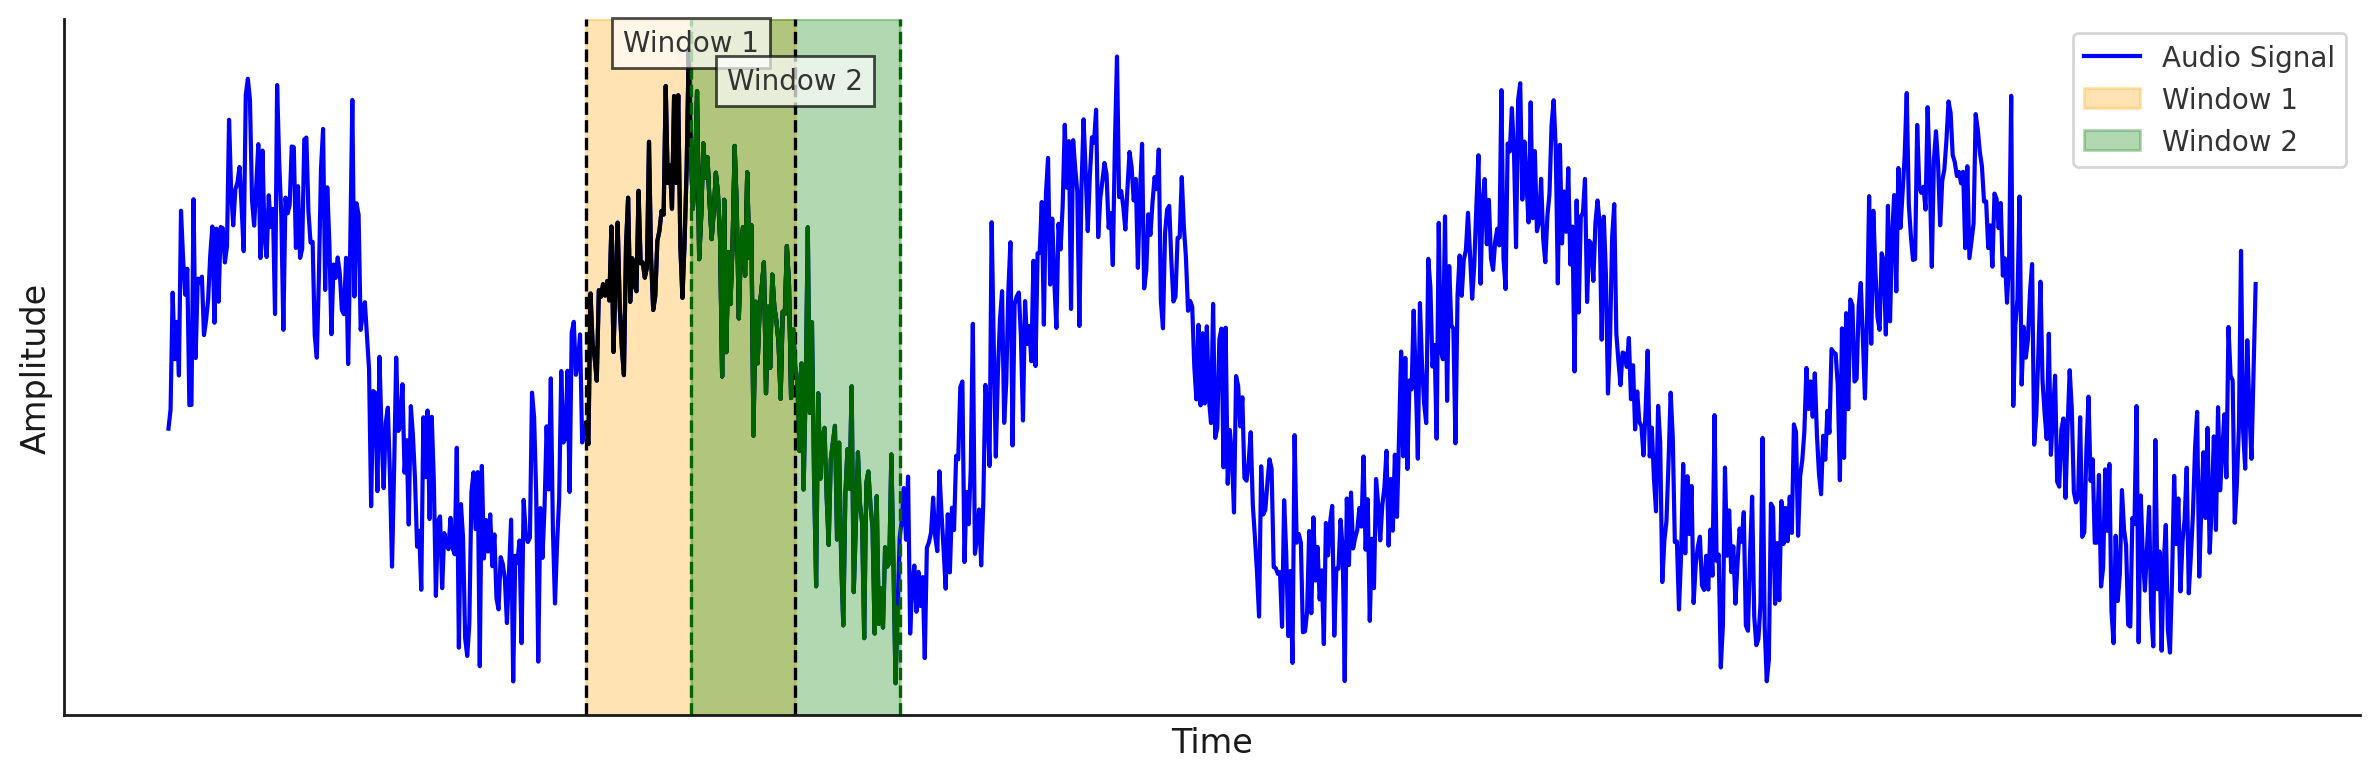
\includegraphics[width=0.8\linewidth]{Chapters/struktura_sustava/generiranje_znacajki/sliding.png} 
    \caption{Preklapajući prozori}
    \label{pic:sliding}
\end{figure}

U glavnoj petlji programskog koda inicijalizirano je polja koje sprema nove uzorke te 
polje koje zaduženo za spremanje trenutnog prozora podataka. Alokacija polja i algoritam
pomicanja starih podataka u polju koje sprema trenutni prozor prikazani su u isječku programskog
koda \ref{code:sliding}.

\begin{lstlisting}[language=C, caption=Sliding Window with Overlap]
    int16_t newSamples[STEP_SIZE];
    int16_t audioFrame[WINDOW_SIZE] = {0};
    
    /**
    * Sliding window with overlap. Audio frame holds WINDOW_SIZE samples.
    * Each update shifts "Samples to Keep" to the start of the buffer,
    * discards "Old Samples" and makes space at the end for "New Samples."
    *
    * Before:
    * -------------------------------------------------------------
    * | Old Samples           | Samples to Keep                   |
    * -------------------------------------------------------------
    * |<----- STEP_SIZE ----->|<---- WINDOW_SIZE - STEP_SIZE ---->|
    * -------------------------------------------------------------
    *
    * After:
    * -------------------------------------------------------------
    * | Kept Samples                      | New Samples           |
    * -------------------------------------------------------------
    * |<---- WINDOW_SIZE - STEP_SIZE ---->|<----- STEP_SIZE ----->|
    * -------------------------------------------------------------
    */
    memcpy(audioFrame, audioFrame + STEP_SIZE, (WINDOW_SIZE - STEP_SIZE) * 2);
    memcpy(audioFrame + WINDOW_SIZE - STEP_SIZE, newSamples, STEP_SIZE * 2);
\end{lstlisting}
\label{code:sliding}

WINDOW\_SIZE predstavlja konfigurabilnu veličinu prozora, dok STEP\_SIZE predstavlja 
konfigurabilni broj novih uzoraka koji će biti dohvaćeni (veličina koraka prozora).
Spomenute konstante, kao i ostali konfigurabilni parametri, definirani su u 
datoteci Configuration.hpp, a prikazani u dodatku \ref{add:config}.

\subsubsection{Funkcija vremenskog otvora}
Nakon što je ustanovljen način dohvaćanja sirovih zvučnih uzoraka, potrebno je
nad pojedinačnim prozorom podataka napraviti sve što je potrebno kako bismo
dobili MFC koeficijente za takav zvučni isječak. Prva stvar koja dolazi na red 
je primjena funkcije vremenskog otvora (engl. window function). Budući da je svaki
prozor (vremenski otvor) podataka opisan u \ref{sec:win} jednostavno odrezan od ostatka
signala, tj. svega što je ostalo izvan prozora, dolazi do rasipanja energije po
frekvencijskom sprektru ili spektralnog curenja (engl. spectral leakage). 
Zbog toga je potrebno pomnožiti originalni signal s funkcijom vremenskog prozora. Postoje
različite funkcije koje se koriste u tu svrhu, međutim u obradi govora najčešće se koristi
Hannov prozor \cite{windowing}.
Na slici \ref{pic:hann} prikazan je umnožak funkcije Hannovog prozora s funkcijom
koja predstavlja zvučni signal. Na konačnom signalu je vidljivo da se rubni dijelovi
signala vrijednostima približavaju nuli što sprječava diskontinuiranost signala i pojavu 
nepoželjnih spektralnih komponenti.

\begin{figure}[htb]
    \centering
    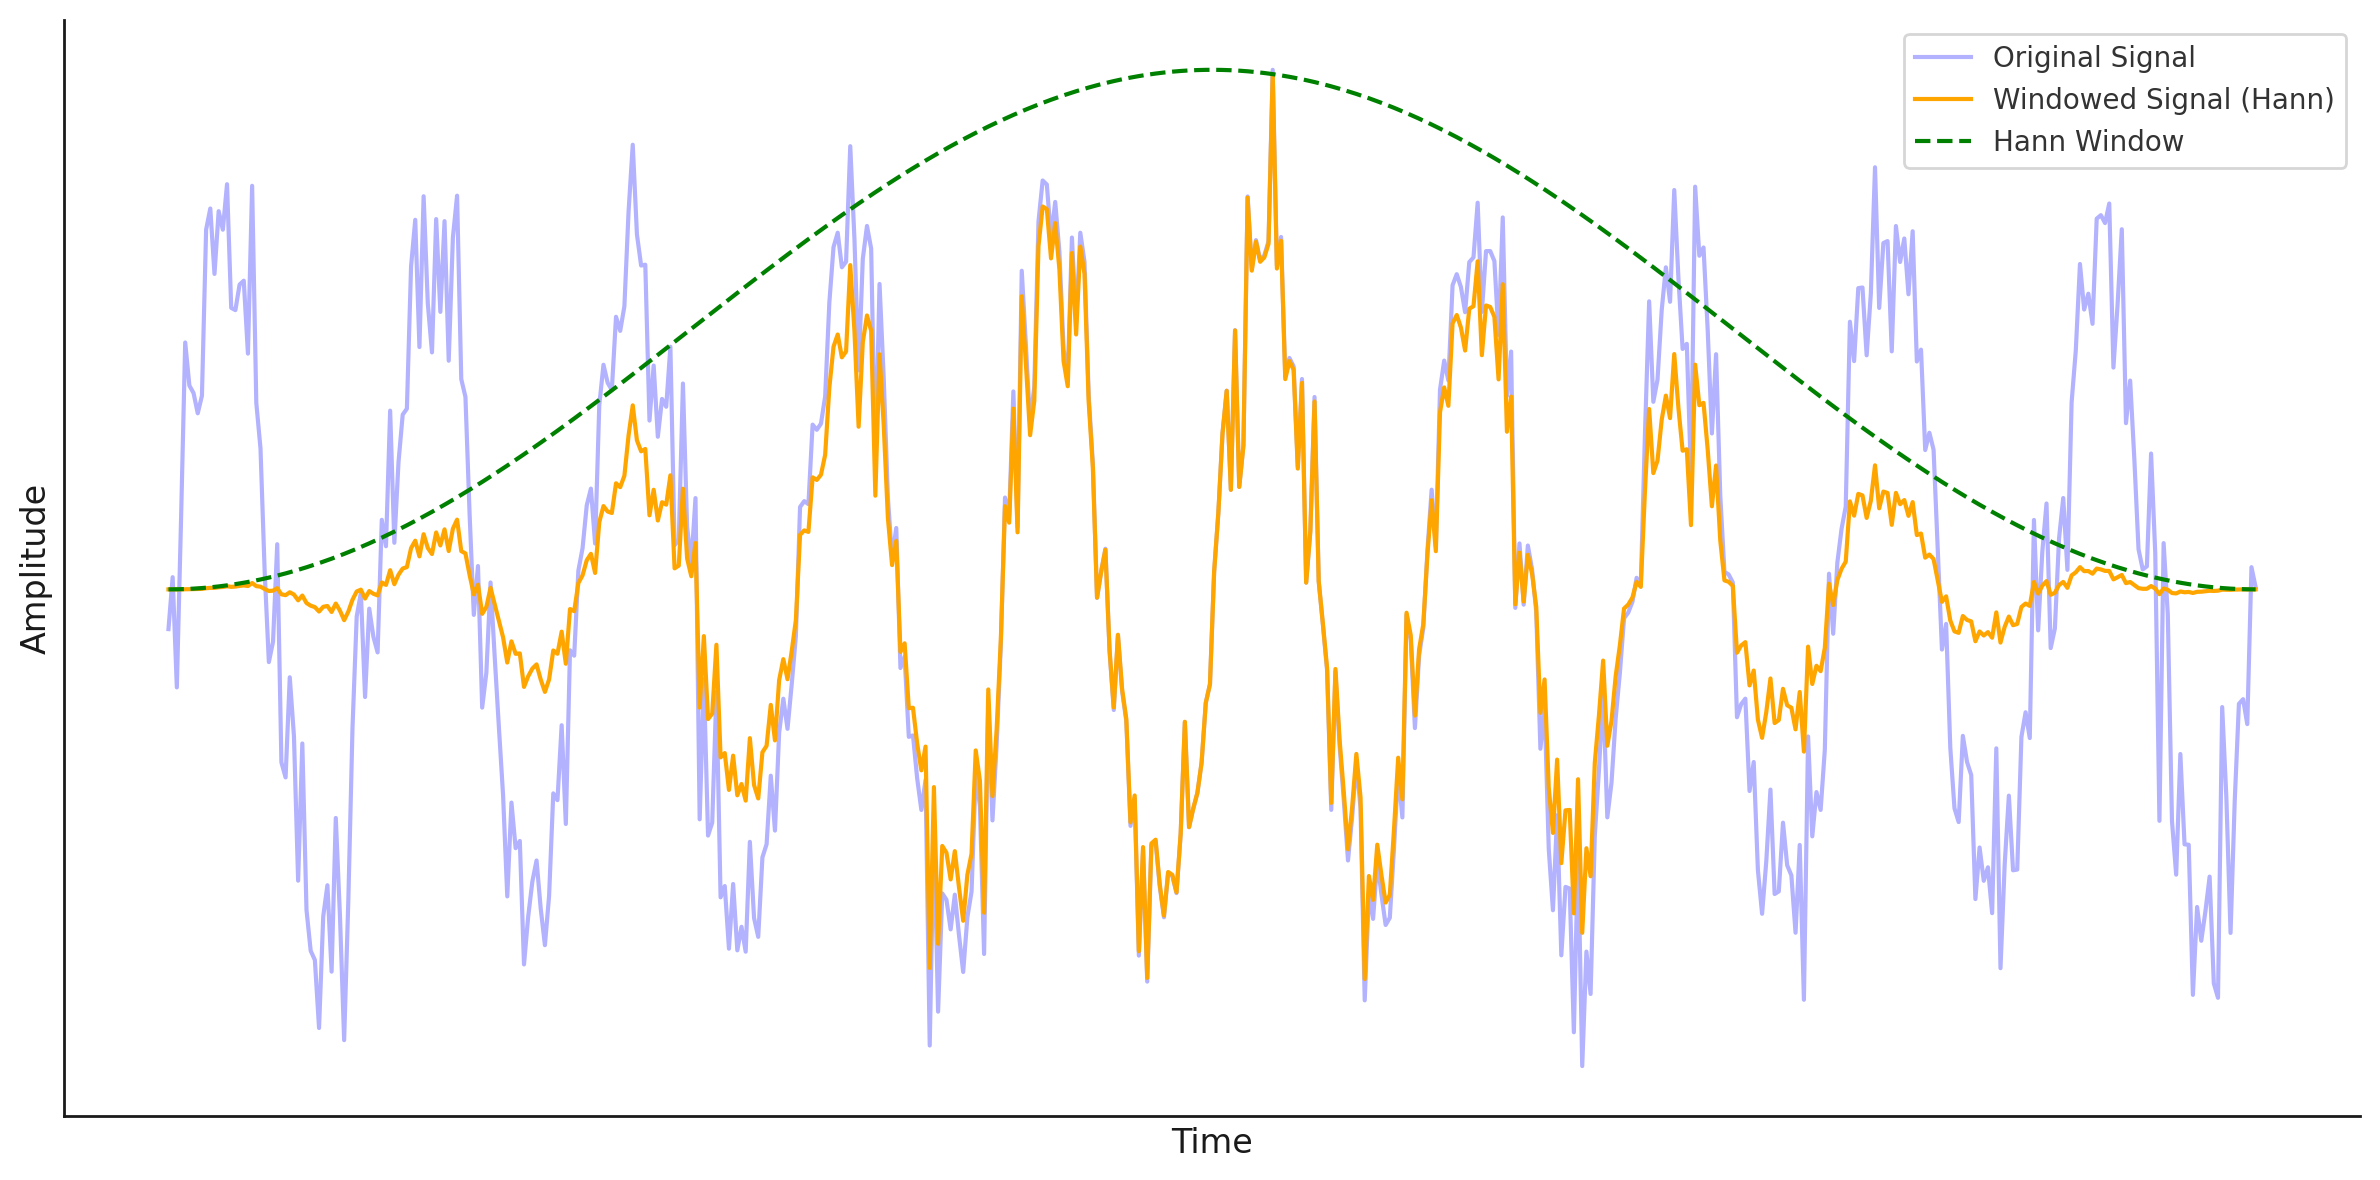
\includegraphics[width=0.8\linewidth]{Chapters/struktura_sustava/generiranje_znacajki/hann.png} 
    \caption{Hannov prozor}
    \label{pic:hann}
\end{figure}

Opisani postupak množenja originalnog signala Hannovim prozorom prikazan je 
matematičkim izrazom \ref{eq:window}.

\begin{equation}
    \label{eq:window}
    x_w[n] = x[n] \cdot w[n]
\end{equation}

gdje je:
\begin{itemize}
    \item \( x_w[n] \) signal nakon primjene Hann prozora,
    \item \( x[n] \) originalni diskretni signal,
    \item \( w[n] \) Hann prozor definiran kao:
    \begin{equation}
        w[n] = 0.54 - 0.46 \cdot \cos\left( \frac{2 \pi n}{N-1} \right)
    \end{equation}
    za \( n = 0, 1, 2, \dots, N-1 \),
    gdje je \( N \) ukupni broj uzoraka u prozoru.
\end{itemize}

Dobiveni signal veličine WINDOW\_SIZE je nakon opisane obrade spreman za spektralnu analizu
koja podrazumijeva korištenje diskretne Fourierove transformacije.

\subsubsection{Diskretna Fourierova transformacija}
\label{sec:fft}

Diskretna Fourierova transformacija (engl. Discrete Fourier Transform ili DFT) matematička je
funkcija koja se koristi za analizu diskretnih signala u frekvencijskoj domeni. 
DFT diskretnog signala \( x[n] \) s \( N \) uzoraka definirana je izrazom \ref{eq:dft}.

\begin{equation}
    X[k] = \sum_{n=0}^{N-1} x[n] e^{-j 2 \pi k n / N}, \quad k = 0, 1, \dots, N-1
\end{equation}
\label{eq:dft}
gdje je:
\begin{itemize}
    \item \( X[k] \): spektralni koeficijent na \( k \)-toj frekvenciji,
    \item \( x[n] \): signal u vremenskoj domeni,
    \item \( N \): broj uzoraka signala,
    \item \( e^{-j 2 \pi k n / N} \): osnovni eksponencijalni faktor.
\end{itemize}

Međutim, računalno je zahtjevna te se zbog toga koristi puno brži algoritam izračuna
frekvencijskih komponenata koji se zove Brza Fourierova transformacija (engl. Fast Fourier
Transform ili FFT). To je učinkovita računalna implementacija DFT-a koja značajno smanjuje
broj operacija potrebnih za izračun koeficijenata spektra.

Na mikrokontrolerskom sustavu koji se koristi za implementaciju cjelokupnog sustava
dostupne su funkcije koje izračunavaju spektralne koeficijente za dani signal. 
Programski kod \ref{code:fft} prikazuje inicijalizacijski kod potreban za pravilnu 
upotrebu FFT-a te metodu \texttt{void FFT::compute(float* frame, float* spectrogram)} 
razreda FFT koja izračunava koeficijente koji predstavljaju kvadratnu vrijednost
amplitude svake frekvencijske komponente (spektar snage signala) kojih ima 
WINDOW\_SIZE / 2 + 1 (još definirano kao NUMBER\_OF\_SPECTROGRAM\_BINS). 


\begin{lstlisting}[language=C++, caption=FFT]

    // initialization 
    dsps_fft2r_init_fc32(NULL, WINDOW_SIZE);

    void FFT::compute(float* frame, float* spectrogram)
    {
        for(size_t i = 0; i < WINDOW_SIZE; i++)
        {
            data[2 * i] = frame[i];  // Real part
            data[2 * i + 1] = 0;     // Imaginary part
        }
        // Perform FFT
        dsps_fft2r_fc32_ae32(data, WINDOW_SIZE);
        // Bit reversal
        dsps_bit_rev_fc32_ansi(data, WINDOW_SIZE);
        // Magnitude (power) of each frequency bin
        for(size_t i = 0; i < NUMBER_OF_SPECTROGRAM_BINS; i++)
        {
            float real = data[2 * i];
            float imag = data[2 * i + 1];
            spectrogram[i] = sqrt(real * real + imag * imag);
        }
    }
\end{lstlisting}
\label{code:fft}

\subsubsection{Mel Filterbank}






\subsubsection{DCT}
\subsection{Konstrukcija feature mape}

